%! alt A circle with centre O and five points on it. The tangents at these points form a convex pentagon around the circle. Two neighbouring points of tangency, P and Q, have tangents meeting at the corner V, with right angles marked at P and Q. The exterior angle at V, between the side through P extended beyond V and the side through Q, is marked and equals angle POQ at the centre: in the case drawn, both are 70 degrees.
%! after_paragraph 2
%! scale 8/5
% The shared preamble of every Cevian figure. pipeline/figures turns these colours into theme-aware paint,
% and refuses any other colour, so draw only with them:
%   figink (lines and labels), figaux (construction lines), figaccent (the object the argument turns on),
%   figtint and figaccenttint (light fills).
\documentclass[border=1.5pt]{standalone}
\usepackage{tkz-euclide}
\definecolor{figink}{RGB}{0,0,0}
\definecolor{figaux}{RGB}{85,85,85}
\definecolor{figaccent}{RGB}{192,57,43}
\definecolor{figtint}{RGB}{221,221,221}
\definecolor{figaccenttint}{RGB}{245,213,208}
% tkz-euclide's defaults draw circles, compasses and marks in 50% grey and fill points with a tint.
\makeatletter
\def\tkz@otherlinecolor{figink}
\def\tkz@euc@circlecolor{figink}
\def\tkz@euc@compasscolor{figink}
\def\tkz@euc@mkcolor{figink}
\def\tkz@mk@fill{figink}
\def\tkz@euc@pointfillcolor{figink}
\makeatother
\tkzSetUpLine[color=figink,line width=.7pt]
\tkzSetUpArc[color=figink,line width=.7pt]
\tkzSetUpCompass[color=figink,line width=.5pt]
\tkzSetUpPoint[color=figink,fill=figink,size=3.1pt]
\tikzset{
  every picture/.style={line cap=round,line join=round,color=figink},
  circle style/.append style={color=figink,line width=.7pt},
  aux/.style={color=figaux,line width=.45pt,dash pattern=on 2.6pt off 2pt},
  key/.style={color=figaccent,line width=1pt},
  mk/.style={color=figink,line width=.5pt},
  lbl/.style={color=figink,inner sep=2.2pt},
  len/.style={color=figink,inner sep=1.5pt,font=\small},
}

\begin{document}
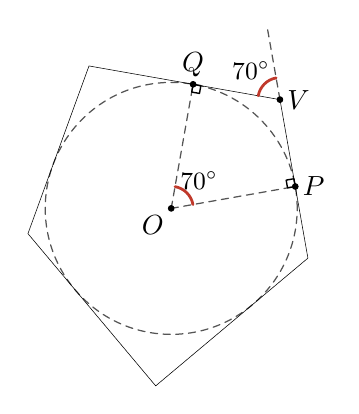
\begin{tikzpicture}
\tkzDefPoint(0.0,0.0){O} %! O = (0, 0)
\tkzDefPoint(1.5756924,0.27783708){P} %! P = polar(O, 1, 10)
\tkzDefPoint(0.27783708,1.5756924){Q} %! Q = polar(O, 1, 80)
\tkzDefPoint(1.3811488,1.3811488){V} %! V = polar(O, 1/cosd(35), 45)
\tkzDefPoint(-1.0443258,1.8088254){Vb} %! Vb = polar(O, 1/cosd(40), 120)
\tkzDefPoint(-1.8194529,-0.32081863){Vc} %! Vc = polar(O, 1/cosd(30), 190)
\tkzDefPoint(-0.19721093,-2.2541313){Vd} %! Vd = polar(O, 1/cosd(45), 265)
\tkzDefPoint(1.7361017,-0.63188935){Ve} %! Ve = polar(O, 1/cosd(30), 340)
\tkzDefPoint(1.2214200,2.2870159){X} %! X = lerp(Ve, V, 1.45)
%! fact on_circle(P, O, 1)
%! fact on_circle(Q, O, 1)
%! fact perp(O, P, P, V)
%! fact perp(O, Q, Q, V)
%! fact collinear(P, Ve, V)
%! fact collinear(Q, V, Vb)
%! fact tangent(O, 1, Vb, Vc)
%! fact tangent(O, 1, Vc, Vd)
%! fact tangent(O, 1, Vd, Ve)
%! fact collinear(X, Ve, V)
%! example angle(P, O, Q) == 70
%! example angle(X, V, Q) == 70
\tkzDrawCircle[aux](O,P)
\tkzDrawSegments[aux](O,P O,Q V,X)
\tkzDrawPolygon(V,Vb,Vc,Vd,Ve)
\tkzMarkRightAngle[size=.1,mk](O,P,V)
\tkzMarkRightAngle[size=.1,mk](V,Q,O)
\tkzMarkAngle[size=.28,arc=l,mark=none,key](P,O,Q)
\tkzMarkAngle[size=.28,arc=l,mark=none,key](X,V,Q)
\tkzLabelAngle[pos=.5,font=\small](P,O,Q){$70^\circ$}
\tkzLabelAngle[pos=.52,font=\small](X,V,Q){$70^\circ$}
\tkzDrawPoints(O,P,Q,V)
\tkzLabelPoint[below left,lbl](O){$O$}
\tkzLabelPoint[right,lbl](P){$P$}
\tkzLabelPoint[above,lbl](Q){$Q$}
\tkzLabelPoint[right,lbl](V){$V$}
\end{tikzpicture}
\end{document}
